\section{El problema de las palabras.}\label{deh}
En esta sección vamos a tratar de ver si dos trenzas dadas son equivalentes entre sí sin hacer uso de invariantes. Vamos a apoyarnos en la idea que vimos en la sección \ref{grupotrenzas}:\\

Consideramos el grupo $ B_{n} $ con la representación que vimos en el teorema \ref{teoBn}. El problema de ver si dos trenzas dadas son equivalentes se puede ver como el problema de las palabras del grupo $ B_{n} $.\\

\textbf{Problema de las palabras del grupo de las trenzas:}\\
Dadas dos palabras de trenzas $\beta1, \beta2 \in B_{n}$ tratamos de encontrar algún método que nos permita confirmar si son o no equivalentes. \\

Ver si dos palabras (de trenzas) dadas $\beta1, \beta2 \in B_{n}$ son equivalentes se pude ver cómo el problema de ver si la palabra $\beta1\beta2^{-1}$ es equivalente a la palabra vacía (trenza trivial). Por tanto el problema de las palabras se puede reducir a distinguir si una palabra es equivalente o no a la palabra vacía. \\

En este proyecto vamos a ver el método de Patrick Dehornoy que nos permite reducir las palabras de trenzas dadas hasta una forma específica que nos permitirá ver si la palabra es igual a la cadena vacía. Para verlo con más detalle necesitamos ver algunas ideas previas.\\

\underline{\textbf{Definición:}}\\
Diremos que una palabra es \textbf{libremente reducida} si no contiene secuencias de la forma $\sigma_{i}^{-1}\sigma_{i} $ ni $\sigma_{i}\sigma_{i}^{-1}$.\\

Por ejemplo, la palabra $\sigma2\sigma1^{-1}\sigma1\sigma3^{-1}$ que representa a la trenza de la figura \ref{deh1} no es libremente reducida pues contiene la palabra $\sigma1^{-1}\sigma1$.\\

	\begin{figure}[h!]
		\centering
		
\includegraphics[width=3cm]{itrenzas/deh1.png}
		\caption{Trenza no libremente reducida.}
		\label{deh1} 
	\end{figure}

\underline{\textbf{Definición:}}\\
Sea la palabra $\beta \in B_{n}$. Llamaremos \textbf{generador principal} de $\beta$ al generador de $\beta$ de menor índice.\\

Por ejemplo, la palabra $\sigma2\sigma1^{-1}\sigma1\sigma3^{-1}$ tiene como generador principal el 1, mientras que la palabra $\sigma2\sigma4^{-1}$ tiene como generador principal el número 2. \\

\textbf{\underline{Definición:}}
Diremos que una palabra $\beta \in B_{n}$ es \textbf{reducida} si se cumple alguna de estas condiciones:
\begin{enumerate}

	\item $\beta$ es la palabra cadena vacía.
	\item El generador principal de $\beta$ se presenta sólo positiva o negativamente. 
\end{enumerate}
 
Por ejemplo, la palabra $\sigma2\sigma1^{-1}\sigma3^{-1}\sigma1$ no es reducida pues el generador principal (1) se encuentra en un cruce negativo y en un cruce positivo. La palabra $\sigma2\sigma1\sigma3^{-1}\sigma1$ si sería reducida pues el generador principal (1) se presenta sólo como cruces positivos.\\

Si tenemos una palabra no reducida con generador principal $ \sigma_{i} $, podemos considerar ocurrencias de la palabra de la forma $ \sigma_{i}^{\pm} ... \sigma_{i}^{\mp} $ que no contengan cruces $ \sigma_{i} $, es decir, entre los cruces de signo opuesto del generador $ \sigma_{i} $ sólo encontramos generadores $ \sigma_{k} $, $ k>i $. Podemos visualizar la idea en la figura \ref{h1}. En este caso diremos que la cadena i+1 forma a\textbf{ handle}.\\
\begin{figure}[h!]
	\centering
	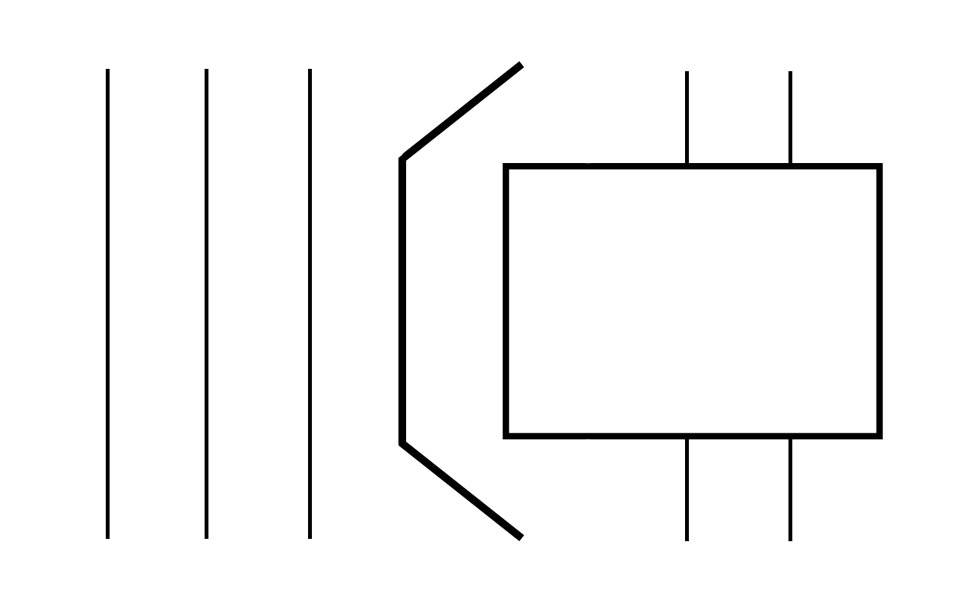
\includegraphics[width=4.5cm]{itrenzas/h11.png}
	\caption{Main handle.}
	\label{h1} 
\end{figure}

\begin{pro}
	Una palabra reducida no vacía no puede ser equivalente a la cadena vacía.
\end{pro}

Por tanto, si encontramos un método para obtener la palabra reducida de una palabra, podremos resolver el problema de las palabras: \\
Si la palabra $\beta1$ reducida es equivalente a la palabra $\beta2$, entonces $\beta2$ es equivalente a la cadena vacía si y sólo si $\beta1$ es la cadena vacía. \\

\begin{pro}
	Cualquier palabra admite una palabra reducida. 
\end{pro}

Para ver una demostración de esta proposición, vamos ir viendo el método que realizaremos para transformar una palabra cualquiera en su palabra reducida.\\ 
Con este método tratamos de eliminar los handles de la trenza, pero para no entrar en bucles infinitos en el algoritmo, vamos a tener que considerar handles generados por cualquier generador y no sólo por el generador principal.\\

\underline{\textbf{Definición:}}\\
 Un \textbf{$ \sigma_{j} $-handle} de una palabra es una sub-palabra de la forma $ \sigma_{j}^{\pm} v \sigma_{j}^{\mp} $ donde la sub-palabra $v$ sólo contiene generadores $\sigma_{k}^{(-1)} $ con k $<$ j-1 o k $>$j. Si el generador $\sigma_{j}$ es el generador principal de la palabra, a dicho $ \sigma_{j} $-handle se conocerá como \textbf{main handle}.\\
 
 Podemos ver un $ \sigma_{j} $-handle en la figura \ref{h2}.\\
 \begin{figure}[h!]
 	\centering
 	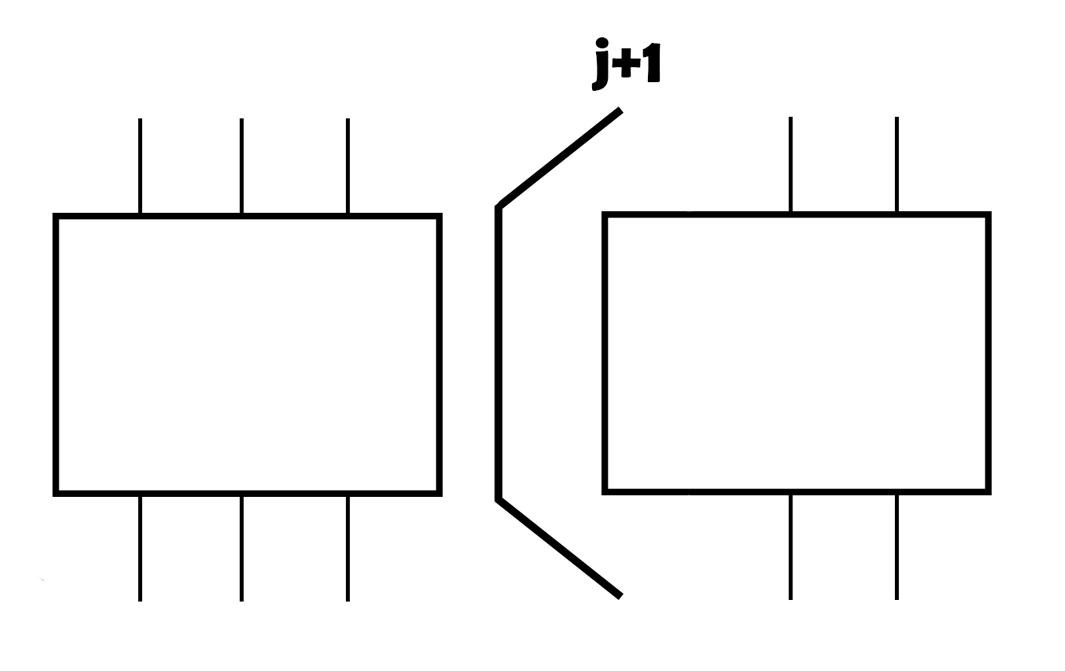
\includegraphics[width=9cm]{itrenzas/h12.png}
 	\caption{A handle.}
 	\label{h2} 
 \end{figure}
 
 Supongamos que tenemos la palabra $ \sigma3\sigma1^{-1}\sigma2\sigma4^{-1}\sigma2^{-1}\sigma4^{-1}\sigma1 $. \\
 La sub-palabra $ \sigma1^{-1}\sigma2\sigma4^{-1}\sigma2^{-1}\sigma4^{-1}\sigma1 $ es un main handle mientras que $\sigma2\sigma4^{-1}\sigma2^{-1} $ es un $ \sigma2 $-handle.\\
 
\underline{\textbf{ Definición:}}\\
Sea $\sigma_{j}^{e}$ $v$ $\sigma_{j}^{-e} $ un $\sigma_{j}$-handle de una palabra $\beta$, donde $e \in$ $ \{-1,1\} $. En particular, podemos denotar dicho $\sigma_{j}$-handle como la siguiente sub-palabra:
\begin{center}
	$ \sigma_{j}^{e} $ $ v_{0} $ $\sigma_{j+1}^{d_{1}} $ $ v_{1}...v_{m-1} $ $\sigma_{j+1}^{d_{m}} $ $ v_{m} $ $ \sigma_{j}^{-e} $
\end{center} donde $v_{0},...,v_{m}$ no contienen generadores $\sigma_{k}^{(-1)}$ con $ j-1 \le k \le j+1 $, $d_{i} \in$ $ \{-1,1\} $\\
Podemos aplicarle una \textbf{reducción local} quedando la sub-palabra equivalente:
\begin{center}
 $ v_{0} $ $\sigma_{j+1}^{-e} \sigma_{j}^{d_{1}} \sigma_{j+1}^{e}$ $ v_{1}...v_{m-1} $ $\sigma_{j+1}^{-e} \sigma_{j}^{d_{m}} \sigma_{j+1}^{e}$ $ v_{m} $
\end{center}
En definitiva hemos aplicado el homomorfismo $\phi_{j,e}$ definido como:
\begin{center}
	$\sigma_{j}^{\pm 1} \rightarrow \epsilon$\\
	$\sigma_{j+1}^{\pm 1} \rightarrow \sigma_{j+1}^{-e} \sigma_{j}^{\pm 1} \sigma_{j+1}^{e}$\\
	$\sigma_{k}^{\pm 1} \rightarrow \sigma_{k}^{\pm 1},$ siendo k$ \neq $j,j+1.\\
\end{center}

Podemos ver esta transformación en la figura \ref{h3}.\\
\begin{figure}[h!]
	\centering
	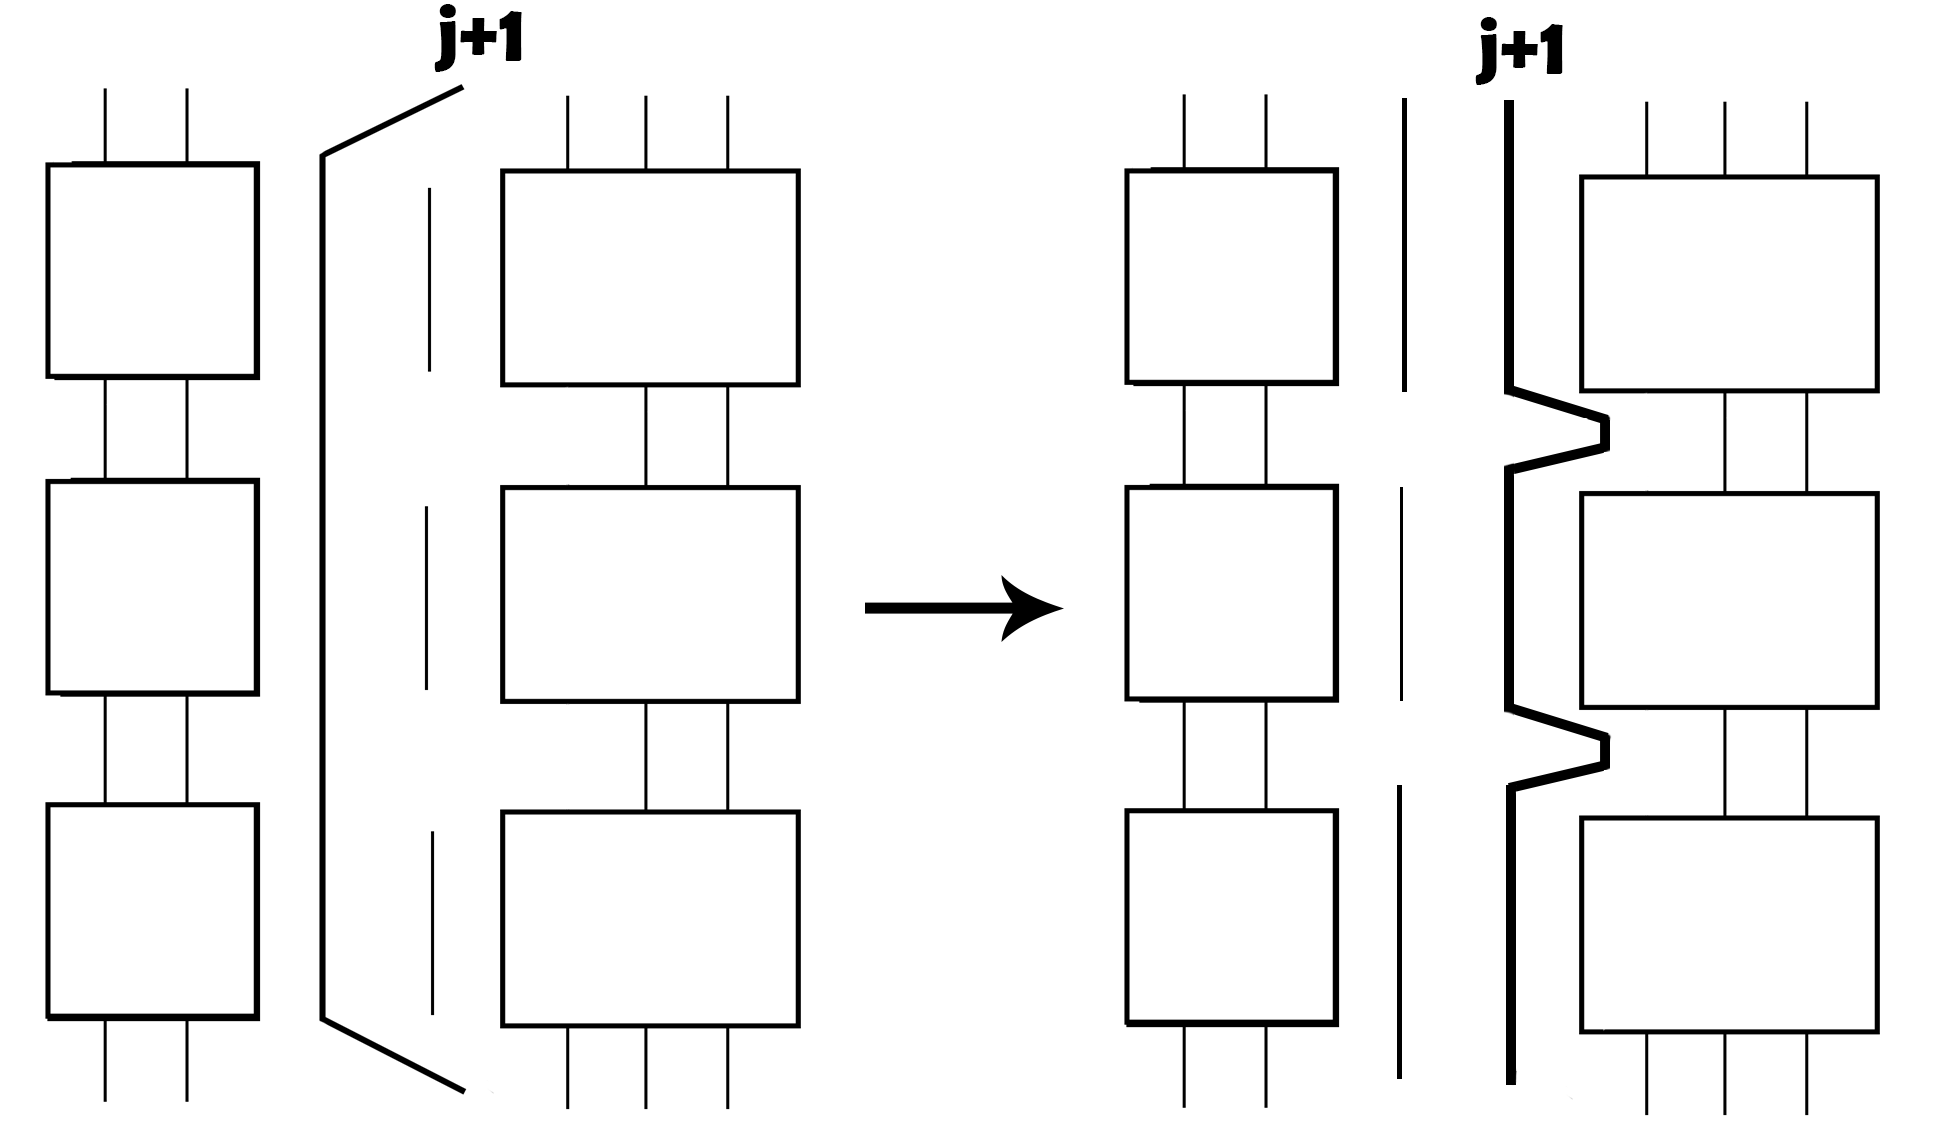
\includegraphics[width=14cm]{itrenzas/h14.png}
	\caption{Reducción local.}
	\label{h3} 
\end{figure}

Es importante destacar que antes de realizar una reducción local a una palabra, tendremos que asegurarnos de que dicha palabra sea libremente reducida para evitar una mayor complejidad.\\

Sea la palabra $\sigma2\sigma1^{-1}\sigma2\sigma3\sigma1$. Podemos aplicar una reducción local al main handle $\sigma1^{-1}\sigma2\sigma3\sigma1$ quedando la palabra $\sigma2\sigma1\sigma2^{-1}\sigma3$. Esta sería su palabra reducida.\\

Pero antes de hacer una reducción local a un $\sigma_{j}$-handle, tendremos que asegurarnos que no tenemos ningún $\sigma_{j+1}$-handle en el $\sigma_{j}$-handle. En el caso de tenerlo, tendríamos que aplicar la reducción local a este $\sigma_{j+1}$-handle y posteriormente aplicar la reducción local al $\sigma_{j}$-handle. De este modo podremos evitar ciclos infinitos. Veámoslo con un ejemplo:\\

Supongamos que queremos obtener la palabra reducida de la palabra $\sigma1\sigma2\sigma3\sigma2^{-1}\sigma1^{-1}$. El generador principal es 1 y tenemos un main handle (que, en este caso, es toda la palabra en sí misma). Aplicamos una reducción local a este main handle quedando: \\
$\sigma2^{-1}\sigma1\sigma2\sigma3\sigma2^{-1}\sigma1^{-1}\sigma2$.
Vemos que volvemos a tener un main handle y entraremos en bucle infinito. Veamos cómo aplicaríamos la solución que hemos comentado:\\

Supongamos de nuevo que queremos obtener la palabra reducida de la palabra $\sigma1\sigma2\sigma3\sigma2^{-1}\sigma1^{-1}$. Tenemos un main handle pero dicho main handle consta de una sub-palabra $\sigma2$-handle. Aplicamos una reducción local a este $\sigma2$-handle quedando:\\
$\sigma1\sigma3^{-1}\sigma2\sigma3\sigma1^{-1}$. Ahora sí podemos aplicar una reducción local al main handle quedando la palabra reducida: \\
$\sigma3^{-1}\sigma2^{-1}\sigma1\sigma2\sigma3$.\\

\underline{\textbf{Definición:}} \\
Diremos que un  $\sigma_{j}$-handle está permitido si no contiene ningún $\sigma_{j+1}$-handle.\\

Por ejemplo el main handle $\sigma1\sigma2\sigma3\sigma2^{-1}\sigma1^{-1}$ no está permitido porque incluye al $\sigma2$-handle $\sigma2\sigma3\sigma2^{-1}$. Este 2-handle sí estaría permitido porque no incluye ningún $\sigma3$-handle. \\

Si un $\sigma_{j}$-handle no está permitido, le aplicaremos reducciones locales, como hemos hecho en el ejemplo, hasta que pase a estar permitido.\\

\underline{\textbf{Definición:}} \\
Diremos que una palabra $\beta'$ es deducida de una palabra $\beta$ usando una \textbf{reducción de handle} si $\beta'$ se obtiene a partir de una reducción local de un $\sigma_{j}$-handle permitido de $\beta$.\\

\begin{teo}
	Cualquier palabra puede ser reducida por una secuencia finita de reducciones de handle hasta llegar a su palabra reducida.
\end{teo}

\bigskip
Para poner en uso todas estas ideas vamos a ver un ejemplo en el que demostraremos que dos palabras dadas son equivalentes:\\
Supongamos que tenemos las palabras $\beta1=\sigma2\sigma3^{-1}\sigma1\sigma2^{-1}\sigma3$ y $\beta2=\sigma1\sigma2\sigma3^{-1}\sigma1\sigma2^{-1}$ que representan a las trenzas de la figura \ref{h4}.\\

\begin{figure}[h!]
	\centering
	\subfigure[$\beta1$]{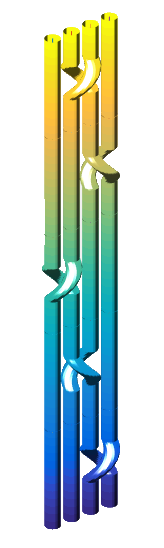
\includegraphics[width=2.3cm]{itrenzas/deho2.png}}
	\subfigure[$\beta2$]{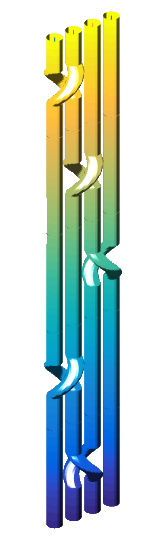
\includegraphics[width=2.2cm]{itrenzas/deho1.png}}
	\caption{Trenzas equivalentes.}
	\label{h4} 
\end{figure}

A simple vista es difícil saber si las palabras son o no equivalentes. Para ver que las palabras son equivalentes ($\beta1 \sim \beta2$), tenemos que ver que se verifica $\beta1 \beta2^{-1} \sim \epsilon$, donde $\epsilon$ representa a la cadena vacía.\\

En primer lugar vamos a considerar la palabra con la que vamos a trabajar:\\
$\beta1 \beta2^{-1} =\sigma2\sigma3^{-1}\sigma1\sigma2^{-1}\sigma3\sigma2\sigma1^{-1}\sigma3\sigma2^{-1}\sigma1^{-1}$.\\

Nos encontramos el main handle $ \sigma1\sigma2^{-1}\sigma3\sigma2\sigma1^{-1} $. Vamos a aplicarle una reducción local, pero vemos que contiene al $\sigma2$-handle $\sigma2^{-1}\sigma3\sigma2$. Por tanto aplicamos una reducción local a este $\sigma2$-handle:\\
$\sigma2^{-1}\sigma3\sigma2$ $\rightarrow$ $\sigma3\sigma2\sigma3^{-1}$, obteniendo la palabra:\\
$\beta1 \beta2^{-1} =\sigma2\sigma3^{-1}\sigma1\sigma3\sigma2\sigma3^{-1}\sigma1^{-1}\sigma3\sigma2^{-1}\sigma1^{-1}$.\\

Nos encontramos el main handle permitido $\sigma1\sigma3\sigma2\sigma3^{-1}\sigma1^{-1}$. Le aplicamos una reducción local:\\ 
$\sigma1\sigma3\sigma2\sigma3^{-1}\sigma1^{-1}$ $\rightarrow$ $\sigma3\sigma2^{-1}\sigma1\sigma2\sigma3^{-1}$, obteniendo la palabra:\\
$\beta1 \beta2^{-1} =\sigma2\sigma3^{-1}\sigma3\sigma2^{-1}\sigma1\sigma2\sigma3^{-1}\sigma3\sigma2^{-1}\sigma1^{-1}$.\\

Esta palabra no es libremente reducida porque nos encontramos un par de veces la sub-palabra $ \sigma3^{-1}\sigma3 $. Las eliminamos y obtenemos la palabra:\\
$\beta1 \beta2^{-1} =\sigma2\sigma2^{-1}\sigma1\sigma2\sigma2^{-1}\sigma1^{-1}$.\\

De nuevo nos encontramos con una palabra que no es libremente reducida porque nos encontramos un par de veces la sub-palabra $ \sigma2\sigma2^{-1} $. Las eliminamos y obtenemos la palabra:\\
$\beta1 \beta2^{-1} =\sigma1\sigma1^{-1}$.\\

Otra vez nos encontramos con una palabra no libremente reducida. Eliminamos la sub-palabra $\sigma1\sigma1^{-1}$ quedando la cadena vacía, es decir:\\
$\beta1 \beta2^{-1} =\epsilon$.\\

Concluimos que ambas palabras son equivalentes, luego las trenzas a las que representan son equivalentes. Sus trenzas cerradas serán equivalentes y por tanto los nudos a los que se está representando son también equivalentes.\\
